\lecture{3}{29 Sep.}{}

\begin{recall}
    A tournament \(T\) is an orientation of \(K_n\), and it has the \(k\)-Sch\"utte property if no \(k\) of its vertices jointly beat everyone else: for every \(U \subseteq V(T)\) with \(\abs{U} = k\) there is a vertex \(v \notin U\) beating every \(u \in U\). For \(k = 1\) this says that there is no winner.
\end{recall}

\autoref{sec:schutte} ended by asking how small a tournament with the \(k\)-Sch\"utte property can be. This lecture answers that question up to a polynomial factor, by the same pair of techniques used for \(m(k)\) in \autoref{sec:property-B}: a deterministic greedy argument for the lower bound, and a random construction with a union bound for the upper bound.

\subsection{The Extremal Function}

\begin{definition}\label{def:f-schutte}
    Let \(f_S(k)\) be the smallest \(n\) s.t.\ there is an \(n\)-vertex tournament with the \(k\)-Sch\"utte property.\footnote{Here \(n > k\) is understood: if \(n < k\) there is no \(k\)-set of vertices at all and the condition holds vacuously, and if \(n = k\) the only \(k\)-set is \(V(T)\), which has no vertex outside it.}
\end{definition}

Since adding a vertex to a tournament with the \(k\)-Sch\"utte property preserves the property (an old witness \(v\) for an old \(k\)-set \(U\) still works), tournaments with the \(k\)-Sch\"utte property exist on every \(n \ge f_S(k)\), and \(f_S(k)\) is the threshold above which they appear.

\begin{eg}\label{eg:fs-one}
    \(f_S(1) = 3\). No tournament on \(1\) or \(2\) vertices has the \(1\)-Sch\"utte property: on one vertex \(v\), the set \(U = \{v\}\) has no vertex outside it; on two vertices, one of them beats the other and is therefore a winner. The cyclic triangle has it, since each of its three vertices is beaten by another one.
    \begin{center}
        \begin{tikzpicture}[thick, >={Stealth[length=6pt]}]
            \coordinate (a) at (90:0.8);
            \coordinate (b) at (210:0.8);
            \coordinate (c) at (330:0.8);
            \draw[->, shorten >=3pt, shorten <=3pt] (a) -- (b);
            \draw[->, shorten >=3pt, shorten <=3pt] (b) -- (c);
            \draw[->, shorten >=3pt, shorten <=3pt] (c) -- (a);
            \foreach \p in {a,b,c} \fill (\p) circle (2.2pt);
        \end{tikzpicture}
    \end{center}
\end{eg}

To work with the \(k\)-Sch\"utte property we name the set of vertices that a given set fails to dominate.

\begin{notation}
    Given a tournament \(T\) and a subset \(X \subseteq V(T)\) of its vertices, let
    \[
        S(X) \coloneqq \{ v \in V(T) : (v, x) \in E(T) \ \forall\, x \in X \},
    \]
    i.e.\ \(S(X)\) is the set of vertices that beat everything in \(X\).
\end{notation}

\begin{center}
    \begin{tikzpicture}[thick, >={Stealth[length=6pt]}, every node/.style={font=\small}]
        % X on the left
        \draw (0,0) ellipse (0.45 and 1.15);
        \foreach \y in {0.75,0.35,-0.75} \fill (0,\y) circle (2pt);
        \node at (0,-0.2) {$\vdots$};
        \node at (0,-1.95) {$X$, \ $\abs{X} = k$};
        % V(T) \ X on the right
        \draw (4.0,0) ellipse (1.8 and 1.6);
        \node at (4.0,-1.95) {$V(T) \setminus X$};
        % S(X) inside
        \fill[blue!10] (3.5,0.35) ellipse (0.95 and 0.9);
        \draw[blue!60!black] (3.5,0.35) ellipse (0.95 and 0.9);
        \node[blue!60!black] at (3.5,-0.2) {$S(X)$};
        \fill (3.95,0.8) circle (2pt);
        \fill[red!80!black] (3.0,0.75) circle (2.4pt);
        \node[right=2pt, red!80!black] at (3.0,0.75) {$v$};
        \foreach \y in {0.75,0.35,-0.75}
            \draw[->, red!80!black, shorten >=3.5pt, shorten <=3.5pt] (3.0,0.75) -- (0,\y);
        \fill (5.1,-0.6) circle (2pt);
        \fill (4.3,-1.05) circle (2pt);
        \fill (2.85,-0.8) circle (2pt);
    \end{tikzpicture}
\end{center}

A vertex \(v\) lies in \(S(X)\) exactly when all \(k\) arcs between \(v\) and \(X\) point away from \(v\), as drawn in red. Note that \(S(\emptyset) = V(T)\), that \(S\) is order-reversing, i.e.\ \(X \subseteq Y \implies S(Y) \subseteq S(X)\), and that \(S(X) \cap X = \emptyset\) for \(X \ne \emptyset\), since no vertex beats itself. The \(k\)-Sch\"utte property is now a statement about \(S\).

\begin{lemma}\label{lem:schutte-S}
    \(T\) has the \(k\)-Sch\"utte property \(\iff\) \(S(X) \ne \emptyset\) for all \(X \subseteq V(T)\) with \(\abs{X} = k\).
\end{lemma}

Both bounds below are proved through this reformulation. In particular, to show \(f_S(k) > n\) we must rule out all \(n\)-vertex tournaments at once:
\begin{align*}
    f_S(k) > n
    &\iff \text{no \(n\)-vertex tournament has the \(k\)-Sch\"utte property} \\
    &\iff \text{every \(n\)-vertex tournament has a set \(X\) of size \(k\) with \(S(X) = \emptyset\).}
\end{align*}
So for the lower bound we are handed an arbitrary tournament and must \emph{find} a bad \(k\)-set in it, which is what the next subsection does greedily.

\subsection{Lower Bound: A Greedy Argument}

The whole argument rests on the following averaging observation.

\begin{lemma}\label{lem:half-wins}
    In any tournament, there is a vertex that wins at least half of its games.
\end{lemma}

\begin{proof}
    Count the total number of wins in a tournament \(T\) on \(n\) vertices. Every game produces exactly one winner, and there are \(\binom{n}{2}\) games, so
    \[
        \sum_{v \in V(T)} \#\{\text{wins of } v\} = \binom{n}{2}.
    \]
    Since there are \(n\) vertices, the average number of wins per vertex is
    \[
        \frac{\binom{n}{2}}{n} = \frac{n-1}{2},
    \]
    and some vertex is at least average, i.e.\ there is a vertex winning at least \(\frac{n-1}{2}\) of the \(n - 1\) games it plays.
\end{proof}

\begin{proposition}\label{prop:fs-lower}
    \(f_S(k) \ge 2^k\).
\end{proposition}

The idea is to build a bad \(k\)-set \(X\) one vertex at a time, choosing at each step a vertex that halves \(S(X)\). Since \(S(\emptyset) = V(T)\) has \(n\) elements, after \(k\) steps at most \(n/2^k\) vertices are left, and if \(n < 2^k\) there are none.
\begin{center}
    \begin{tikzpicture}[thick, >={Stealth[length=5pt]}, every node/.style={font=\small}]
        \draw (0,0.1) rectangle (1.1,2.5);
        \node[align=center] at (0.55,-0.5) {$S(X_0) = V(T)$\\$n$};
        \draw (2.3,0.7) rectangle (3.4,1.9);
        \node[align=center] at (2.85,-0.5) {$S(X_1)$\\$\le \frac{n}{2}$};
        \draw (4.6,1.0) rectangle (5.7,1.6);
        \node[align=center] at (5.15,-0.5) {$S(X_2)$\\$\le \frac{n}{4}$};
        \draw (6.9,1.15) rectangle (8.0,1.45);
        \node[align=center] at (7.45,-0.5) {$S(X_k)$\\$\le \frac{n}{2^k}$};
        \draw[->, red!80!black] (1.25,1.3) -- (2.15,1.3);
        \node[above, red!80!black] at (1.7,1.34) {$v_1$};
        \draw[->, red!80!black] (3.55,1.3) -- (4.45,1.3);
        \node[above, red!80!black] at (4.0,1.34) {$v_2$};
        \draw[->, red!80!black] (5.85,1.3) -- (6.75,1.3);
        \node[above, red!80!black] at (6.3,1.34) {$\cdots$};
    \end{tikzpicture}
\end{center}

\begin{proof}
    Let \(T\) be any tournament on \(n < 2^k\) vertices; by \autoref{lem:schutte-S} it suffices to produce a set \(X\) of \(k\) vertices with \(S(X) = \emptyset\). Start with \(X_0 = \emptyset\), so that \(S(X_0) = V(T)\), and repeat the following for \(i = 1, 2, \ldots, k\).

    If \(S(X_{i-1}) = \emptyset\) already, stop. Otherwise apply \autoref{lem:half-wins} to the tournament \(T[S(X_{i-1})]\) induced by \(T\) on \(S(X_{i-1})\):
    \begin{itemize}
        \item find a vertex \(v_i \in S(X_{i-1})\) beating at least half of the other vertices of \(S(X_{i-1})\);
        \item add it to the set, \(X_i \coloneqq X_{i-1} \cup \{v_i\}\);
        \item this shrinks \(S\) to those vertices of \(S(X_{i-1})\) that beat \(v_i\), since
        \[
            S(X_i) = S(X_{i-1}) \cap \{u : u \text{ beats } v_i\}.
        \]
    \end{itemize}
    Writing \(s = \abs{S(X_{i-1})}\), the vertex \(v_i\) beats at least \(\frac{s-1}{2}\) of the remaining \(s - 1\) vertices, so at most \(\frac{s-1}{2}\) of them beat \(v_i\), and \(v_i \notin S(X_i)\). Hence \(S(X)\) shrinks by a factor of at least \(\frac{1}{2}\) every round:
    \[
        \abs{S(X_i)} \le \frac{\abs{S(X_{i-1})} - 1}{2} \le \frac{\abs{S(X_{i-1})}}{2}.
    \]
    After \(k\) rounds, \(\abs{X_k} = k\) and
    \[
        \abs{S(X_k)} \le \frac{\abs{V(T)}}{2^k} = \frac{n}{2^k} < 1,
    \]
    so \(S(X_k) = \emptyset\). If instead the process stopped early, at some \(X_i\) with \(i < k\) and \(S(X_i) = \emptyset\), extend \(X_i\) to any \(k\)-set \(X \supseteq X_i\); as \(S\) is order-reversing, \(S(X) \subseteq S(X_i) = \emptyset\). Either way \(T\) fails the \(k\)-Sch\"utte property, so \(f_S(k) \ge 2^k\).
\end{proof}

\subsection{Upper Bound: A Random Tournament}

For the upper bound we must exhibit one tournament with the \(k\)-Sch\"utte property. As in \autoref{thm:m-upper-random}, we do not construct it: we choose a tournament at random and show that it has the property with positive probability.

\begin{theorem}[Erd\H{o}s]\label{thm:fs-upper}
    If \(\binom{n}{k} \left( 1 - 2^{-k} \right)^{n-k} < 1\), then \(f_S(k) \le n\).
\end{theorem}

\begin{proof}
    We consider a uniformly random tournament on the vertices \([n] = \{1, 2, \ldots, n\}\), i.e.\ for every pair \(\{i, j\}\) we choose the arc \((i, j)\) or \((j, i)\) uniformly and independently of all other pairs. By \autoref{lem:schutte-S}, the bad events are indexed by the \(k\)-sets \(X\), the event for \(X\) being that \(S(X) = \emptyset\); we bound each one and take a union bound.

    Fix \(X\) with \(\abs{X} = k\) and a vertex \(v \in V \setminus X\). The vertex \(v\) lies in \(S(X)\) iff all \(k\) arcs between \(v\) and \(X\) point away from \(v\), and these \(k\) coin flips are independent, so
    \[
        \mathbb{P}(v \in S(X)) = \mathbb{P}(v \text{ beats all of } X) = \left( \frac{1}{2} \right)^{k}
        \implies \mathbb{P}(v \notin S(X)) = 1 - \frac{1}{2^k}.
    \]
    For distinct \(v \notin X\), the events \(\{v \in S(X)\}\) involve disjoint sets of pairs, namely the \(k\) pairs joining \(v\) to \(X\), hence they are independent. Since \(\abs{V \setminus X} = n - k\),
    \[
        \mathbb{P}(S(X) = \emptyset)
        = \mathbb{P}\bigl( \forall\, v \notin X,\ v \notin S(X) \bigr)
        = \prod_{v \notin X} \mathbb{P}(v \notin S(X))
        = \prod_{v \notin X} \left( 1 - \frac{1}{2^k} \right)
        = \left( 1 - \frac{1}{2^k} \right)^{n-k}.
    \]
    \begin{center}
        \begin{tikzpicture}[thick, >={Stealth[length=6pt]}, every node/.style={font=\small}]
            \draw (0,0) ellipse (0.45 and 1.1);
            \foreach \y in {0.7,0.3,-0.7} \fill (0,\y) circle (2pt);
            \node at (0,-0.22) {$\vdots$};
            \node at (0,-1.95) {$X$, \ $\abs{X} = k$};
            \draw (3.6,0) ellipse (0.5 and 1.35);
            \foreach \y in {0.95,0.5,-0.95} \fill (3.6,\y) circle (2pt);
            \node at (3.6,-0.05) {$\vdots$};
            \node at (3.6,-1.95) {$V \setminus X$, \ $n - k$};
            \draw[->, shorten >=3.5pt, shorten <=3.5pt] (3.6,0.5) -- (0,0.7);
            \draw[->, shorten >=3.5pt, shorten <=3.5pt] (3.6,0.5) -- (0,0.3);
            \draw[->, shorten >=3.5pt, shorten <=3.5pt] (3.6,0.5) -- (0,-0.7);
            \draw[->, gray, shorten >=3.5pt, shorten <=3.5pt] (0,0.7) -- (3.6,0.95);
            \draw[->, gray, shorten >=3.5pt, shorten <=3.5pt] (3.6,0.95) -- (0,-0.7);
            \draw[->, gray, shorten >=3.5pt, shorten <=3.5pt] (0,0.3) -- (3.6,-0.95);
            \node[anchor=west, align=left] at (4.5,0.5)
                {each \(v \notin X\) sees its own \(k\) arcs,\\so the \(n-k\) events are independent};
        \end{tikzpicture}
    \end{center}
    Now take the union bound over all \(\binom{n}{k}\) choices of \(X\):
    \begin{align*}
        \mathbb{P}(T \text{ is not } k\text{-Sch\"utte})
        = \mathbb{P}\bigl( \exists\, X : S(X) = \emptyset \bigr)
        &= \mathbb{P}\Biggl( \bigcup_{X \in \binom{V}{k}} \{S(X) = \emptyset\} \Biggr) \\
        &\le \sum_{X \in \binom{V}{k}} \mathbb{P}(S(X) = \emptyset)
        = \binom{n}{k} \left( 1 - \frac{1}{2^k} \right)^{n-k} < 1
    \end{align*}
    by assumption. Therefore \(\mathbb{P}(T \text{ is } k\text{-Sch\"utte}) > 0\), so there is an \(n\)-vertex tournament with the \(k\)-Sch\"utte property, and \(f_S(k) \le n\).
\end{proof}

It remains to find how small an \(n\) satisfies the hypothesis of \autoref{thm:fs-upper}.

\begin{corollary}\label{cor:fs-upper}
    \(f_S(k) = O(k^2 2^k)\).
\end{corollary}

\begin{proof}
    We estimate the two factors by
    \[
        \binom{n}{k} \le n^k, \qquad \left( 1 - 2^{-k} \right)^{n-k} \le e^{-(n-k)2^{-k}},
    \]
    the second from \(1 - x \le e^{-x}\). So it suffices to have
    \[
        n^k e^{-(n-k)2^{-k}} < 1
        \iff k \ln n - (n - k) 2^{-k} < 0
        \iff n > k 2^k \ln n + k.
    \]
    The right-hand side grows only logarithmically in \(n\), so the inequality holds as soon as \(n\) is a little larger than \(k 2^k \ln n\). Taking \(n = \lceil k^2 2^k \rceil\) gives \(\ln n = k \ln 2 + 2 \ln k + O(1) = (1 + o(1)) k \ln 2\), hence
    \[
        k 2^k \ln n + k = (1 + o(1)) \, (\ln 2) \, k^2 2^k < k^2 2^k \le n
    \]
    for large \(k\), as \(\ln 2 < 1\). Thus \(n = \Theta(k^2 2^k)\) suffices, and \(f_S(k) = O(k^2 2^k)\).
\end{proof}

Putting \autoref{prop:fs-lower} and \autoref{cor:fs-upper} together:

\begin{theorem}
    \(2^k \le f_S(k) \le C k^2 2^k\) for some constant \(C > 0\).
\end{theorem}

\begin{remark}
    This is the same picture as for Property B: an easy greedy lower bound \(2^k\), a random upper bound \(O(k^2 2^k)\), and a gap of a polynomial factor \(O(k^2)\) between them. Compare \(2^{k-1} \le m(k) \le C k^2 2^k\) from \autoref{sec:property-B}, where the lower bound has since been improved to \(c \sqrt{k / \ln k} \, 2^k\).
\end{remark}

\begin{exercise}
    Show that \(f_S(k) \ge c \, k 2^k\) for some constant \(c > 0\), improving \autoref{prop:fs-lower} by a factor of \(k\).
\end{exercise}

\section{The Erd\H{o}s--Ko--Rado Theorem}\label{sec:ekr}

\subsection{Intersecting Families}

Property B asked how to \emph{split} a family of sets; we now ask how large a family can be if no two of its members can be split apart at all, i.e.\ if they pairwise overlap.

\begin{definition}[Intersecting family]
    A family \(\mathcal{F} \subseteq 2^{[n]}\) is \vocab{intersecting} if \(A \cap B \ne \emptyset\) for any two members \(A, B \in \mathcal{F}\).
\end{definition}

\begin{question}
    How large can an intersecting family be?
\end{question}

There are two natural ways to build a large one: take only \emph{big} sets, which are forced to overlap for lack of room, or take only sets through one fixed element.

\begin{eg}[Large sets]\label{eg:ekr-large}
    For \(n \ge 3\), the family \(\mathcal{F} = \{[n]\} \cup \bigl\{ [n] \setminus \{x\} : x \in [n] \bigr\}\) is intersecting, since any two of its members miss at most two elements between them. More generally, take every set of size more than \(\frac{n}{2}\),
    \[
        \mathcal{F} = \binom{[n]}{n} \cup \binom{[n]}{n-1} \cup \cdots \cup \binom{[n]}{\lceil \frac{n+1}{2} \rceil}.
    \]
    If \(\abs{A}, \abs{B} > \frac{n}{2}\) then \(\abs{A} + \abs{B} > n\), so there is not enough space in \([n]\) for \(A\) and \(B\) to be disjoint. For odd \(n\), exactly half of all subsets have size more than \(\frac{n}{2}\), so \(\abs{\mathcal{F}} = 2^{n-1}\).
\end{eg}

\begin{eg}[Stars]\label{eg:ekr-star}
    Fix \(x \in [n]\) and let \(\mathcal{F}_x = \{F \subseteq [n] : x \in F\}\) be the \vocab{star} at \(x\), i.e.\ the family of \emph{all} subsets containing \(x\). Any two members share \(x\), so \(\mathcal{F}_x\) is intersecting, and \(\abs{\mathcal{F}_x} = 2^{n-1}\), since a subset containing \(x\) is determined by its intersection with \([n] \setminus \{x\}\).
\end{eg}

Both examples reach \(2^{n-1}\), and nothing does better.

\begin{proposition}\label{prop:ekr-trivial}
    If \(\mathcal{F} \subseteq 2^{[n]}\) is intersecting, then \(\abs{\mathcal{F}} \le 2^{n-1}\).
\end{proposition}

\begin{proof}
    Partition all \(2^n\) subsets into the \(2^{n-1}\) complementary pairs \(\{F, [n] \setminus F\}\). The two members of a pair are disjoint, so an intersecting family contains at most one set from each pair, whence \(\abs{\mathcal{F}} \le 2^{n-1}\).
\end{proof}

\autoref{eg:ekr-large} is really a cheat: it wins by using only large sets. The question becomes interesting once all sets are required to have the same size.

\begin{question}[Erd\H{o}s--Ko--Rado]\label{q:ekr}
    What is the largest intersecting family \(\mathcal{F} \subseteq \binom{[n]}{k}\)?
\end{question}

If \(n < 2k\), then any two \(k\)-sets \(A, B \subseteq [n]\) satisfy \(\abs{A} + \abs{B} = 2k > n\) and hence intersect, so \(\binom{[n]}{k}\) is itself intersecting and the answer is \(\binom{n}{k}\). \textbf{From now on we assume \(n \ge 2k\).} The star of \autoref{eg:ekr-star}, cut down to \(k\)-sets, still works.

\begin{eg}[The \(k\)-uniform star]\label{eg:ekr-kstar}
    Fix \(x \in [n]\). The \vocab{star} at \(x\) is
    \[
        \mathcal{F}_x^{(k)} \coloneqq \Bigl\{ F \in \tbinom{[n]}{k} : x \in F \Bigr\},
    \]
    the family consisting of \emph{every} \(k\)-set that contains \(x\), and of nothing else. It is intersecting, as any two of its members share \(x\). Choosing a \(k\)-set through \(x\) amounts to choosing its other \(k-1\) elements from \([n] \setminus \{x\}\), so
    \[
        \bigl\lvert \mathcal{F}_x^{(k)} \bigr\rvert = \binom{n-1}{k-1},
        \qquad
        \frac{\bigl\lvert \mathcal{F}_x^{(k)} \bigr\rvert}{\bigl\lvert \binom{[n]}{k} \bigr\rvert} = \frac{k}{n}.
    \]
    In the picture, each ellipse is one member of the star, and they meet exactly in the red element \(x\).
    \begin{center}
        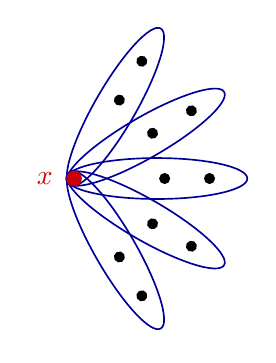
\begin{tikzpicture}[thick]
            \foreach \a in {-60,-30,0,30,60} {
                \draw[blue!60!black, semithick, rotate=\a] (1.05,0) ellipse (1.15 and 0.26);
                \fill[rotate=\a] (1.15,0) circle (2pt);
                \fill[rotate=\a] (1.72,0) circle (2pt);
            }
            \fill[red!80!black] (0,0) circle (2.8pt);
            \node[left=4pt, red!80!black] at (0,0) {$x$};
        \end{tikzpicture}
    \end{center}
\end{eg}

More generally, call a family \(\mathcal{F} \subseteq \binom{[n]}{k}\) \vocab{trivially intersecting} if all of its members share a common element, i.e.\ \(\bigcap_{F \in \mathcal{F}} F \ne \emptyset\). Such a family is certainly intersecting. The two notions are related but not identical: \(\mathcal{F}\) is trivially intersecting exactly when \(\mathcal{F} \subseteq \mathcal{F}_x^{(k)}\) for some \(x\), so the trivially intersecting families are precisely the subfamilies of stars, and the stars are the largest of them. In particular a trivially intersecting family of the full size \(\binom{n-1}{k-1}\) \emph{is} a star.

The Erd\H{o}s--Ko--Rado theorem says that for \(n \ge 2k\) a star is already optimal.

\begin{theorem}[Erd\H{o}s--Ko--Rado, 1961]\label{thm:ekr}
    If \(n \ge 2k\) and \(\mathcal{F} \subseteq \binom{[n]}{k}\) is intersecting, then \(\abs{\mathcal{F}} \le \binom{n-1}{k-1}\).
\end{theorem}

\subsection{Katona's Cycle Method}

The proof we give is Katona's, and it is a probabilistic argument of a shape we have not used yet. Rather than bounding \(\abs{\mathcal{F}}\) directly, we exhibit a random \(k\)-set \(A\) that is uniform on \(\binom{[n]}{k}\), so that \(\mathbb{P}(A \in \mathcal{F}) = \abs{\mathcal{F}} / \binom{n}{k}\), and then bound that same probability by \(\frac{k}{n}\) using a completely different description of \(A\). Comparing the two expressions gives the theorem.

The second description arranges \([n]\) around a circle. Fix \(n\) positions \(1, 2, \ldots, n\) around a circle, and let a \vocab{cyclic permutation} \(\sigma\) of \([n]\) be a placement of the \(n\) elements at those positions, i.e.\ a bijection from positions to elements, with \(\sigma(i)\) the element at position \(i\). There are \(n!\) of them. The word \emph{cyclic} refers to the positions being read modulo \(n\), so that position \(n\) is followed by position \(1\). Call
\[
    I_i^\sigma = \{\sigma(i), \sigma(i+1), \ldots, \sigma(i+k-1)\}, \qquad i \in [n],
\]
with indices read modulo \(n\), the \vocab{intervals of length \(k\)} of \(\sigma\). There are exactly \(n\) of them, one per starting position, and most \(k\)-sets are not intervals of any given \(\sigma\).
\begin{center}
    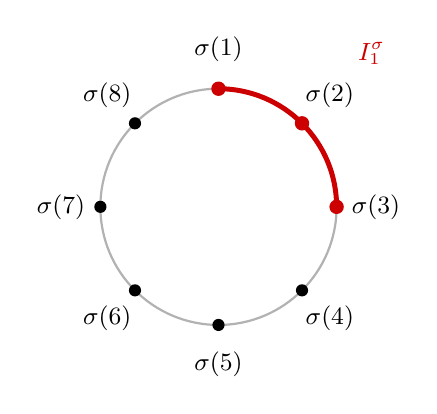
\begin{tikzpicture}[thick, every node/.style={font=\small}]
        \draw[gray!60] (0,0) circle (1.5);
        \foreach \i in {0,...,7} \fill (90-45*\i:1.5) circle (2.2pt);
        \draw[red!80!black, line width=1.8pt] (90:1.5) arc (90:0:1.5);
        \foreach \i in {0,1,2} \fill[red!80!black] (90-45*\i:1.5) circle (2.6pt);
        \foreach \i/\lab in {0/1, 1/2, 2/3, 3/4, 4/5, 5/6, 6/7, 7/8}
            \node at (90-45*\i:2.0) {$\sigma(\lab)$};
        \node[red!80!black] at (45:2.75) {$I_1^\sigma$};
    \end{tikzpicture}
\end{center}

The point of intervals is that a circle has very little room for pairwise intersecting ones.

\begin{lemma}[Katona]\label{lem:katona}
    Let \(n \ge 2k\) and let \(\mathcal{F} \subseteq \binom{[n]}{k}\) be intersecting. Then for any cyclic permutation \(\sigma\) of \([n]\), at most \(k\) of the \(n\) intervals of length \(k\) of \(\sigma\) belong to \(\mathcal{F}\).
\end{lemma}

\begin{proof}
    Fix \(\sigma\). If no interval lies in \(\mathcal{F}\) we are done, so fix an interval \(F \in \mathcal{F}\); after rotating the labels we may assume \(F = \{\sigma(1), \ldots, \sigma(k)\}\).

    First we count the other intervals meeting \(F\). An interval other than \(F\) meets \(F\) exactly when it starts at one of \(\sigma(2), \ldots, \sigma(k)\), or ends at one of \(\sigma(1), \ldots, \sigma(k-1)\). Since \(n \ge 2k\), these \((k-1) + (k-1) = 2k-2\) intervals are distinct and none of them is \(F\).

    Now pair them up. For each \(i\) with \(1 \le i \le k-1\), pair
    \[
        \underbrace{\{\sigma(i-k+1), \ldots, \sigma(i)\}}_{\text{the interval ending at } \sigma(i)}
        \quad \text{with} \quad
        \underbrace{\{\sigma(i+1), \ldots, \sigma(i+k)\}}_{\text{the interval starting at } \sigma(i+1)}.
    \]
    \begin{center}
        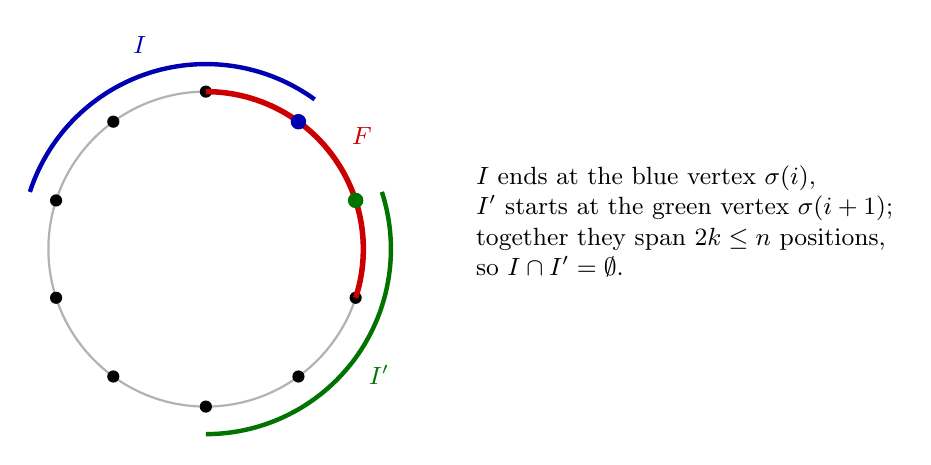
\begin{tikzpicture}[thick, every node/.style={font=\small}]
            \draw[gray!60] (0,0) circle (2);
            \foreach \i in {0,...,9} \fill (90-36*\i:2) circle (2.2pt);
            \draw[red!80!black, line width=2pt] (90:2) arc (90:-18:2);
            \node[red!80!black] at (36:2.45) {$F$};
            \draw[blue!70!black, line width=1.6pt] (162:2.35) arc (162:54:2.35);
            \node[blue!70!black] at (108:2.72) {$I$};
            \fill[blue!70!black] (54:2) circle (2.8pt);
            \draw[green!45!black, line width=1.6pt] (18:2.35) arc (18:-90:2.35);
            \node[green!45!black] at (-36:2.72) {$I'$};
            \fill[green!45!black] (18:2) circle (2.8pt);
            \node[anchor=west, align=left] at (3.3,0.35)
                {\(I\) ends at the blue vertex \(\sigma(i)\),\\\(I'\) starts at the green vertex \(\sigma(i+1)\);\\together they span \(2k \le n\) positions,\\so \(I \cap I' = \emptyset\).};
        \end{tikzpicture}
    \end{center}
    These two intervals occupy \(2k\) consecutive positions of the circle, and \(n \ge 2k\), so they are \emph{disjoint}. Every one of the \(2k-2\) intervals meeting \(F\) occurs in exactly one such pair, so they split into \(k-1\) disjoint pairs.

    Since \(\mathcal{F}\) is intersecting it contains at most one interval from each disjoint pair, and every interval of \(\mathcal{F}\) other than \(F\) must meet \(F\). Hence \(\mathcal{F}\) contains at most \((k-1) + 1 = k\) intervals of \(\sigma\).
\end{proof}

\begin{proof}[Proof of \autoref{thm:ekr}]
    Define a random \(k\)-set \(A \in \binom{[n]}{k}\) as follows.
    \begin{enumerate}[(1)]
        \item Choose a uniformly random cyclic permutation \(\sigma\) of \([n]\).
        \item Choose \(i \in [n]\) uniformly at random, independently of \(\sigma\), and set \(A = I_i^\sigma = \{\sigma(i), \sigma(i+1), \ldots, \sigma(i+k-1)\}\).
    \end{enumerate}
    We first check that \(A\) is uniform on \(\binom{[n]}{k}\). Fix \(S \in \binom{[n]}{k}\) and count the pairs \((\sigma, i)\) with \(I_i^\sigma = S\): the start \(i\) is any of the \(n\) positions, and \(\sigma\) must then place \(S\) at the positions \(i, \ldots, i+k-1\) and \([n] \setminus S\) at the rest, in \(k! \, (n-k)!\) ways. So \(n \cdot k! \, (n-k)!\) pairs produce \(S\), a count not depending on \(S\), and as \((\sigma, i)\) is uniform among all \(n \cdot n!\) pairs,
    \[
        \mathbb{P}(A = S) = \frac{n \cdot k! \, (n-k)!}{n \cdot n!} = \frac{1}{\binom{n}{k}} \quad \text{for every } S.
    \]
    Therefore
    \begin{equation}\tag{1}\label{eq:ekr-one}
        \mathbb{P}(A \in \mathcal{F}) = \frac{\abs{\mathcal{F}}}{\bigl\lvert \binom{[n]}{k} \bigr\rvert} = \frac{\abs{\mathcal{F}}}{\binom{n}{k}}.
    \end{equation}
    On the other hand, condition on \(\sigma\). As \(i\) was chosen independently of \(\sigma\), it is still uniform on \([n]\), so \(A\) is one of the \(n\) intervals of \(\sigma\), each with probability \(\frac{1}{n}\), and
    \[
        \mathbb{P}(A \in \mathcal{F} \mid \sigma) = \frac{\#\{ i \in [n] : I_i^\sigma \in \mathcal{F} \}}{n} \le \frac{k}{n}
        \quad \text{for \emph{every} } \sigma.
    \]
    The inequality is \autoref{lem:katona}: since \(k < n\), distinct starts give distinct intervals, so the numerator counts the intervals of \(\sigma\) lying in \(\mathcal{F}\). Averaging over \(\sigma\),
    \begin{equation}\tag{2}\label{eq:ekr-two}
        \mathbb{P}(A \in \mathcal{F}) = \sum_{\sigma} \mathbb{P}(\sigma) \, \underbrace{\mathbb{P}(A \in \mathcal{F} \mid \sigma)}_{\le \, k/n} \le \frac{k}{n} \sum_{\sigma} \mathbb{P}(\sigma) = \frac{k}{n}.
    \end{equation}
    Comparing \eqref{eq:ekr-one} and \eqref{eq:ekr-two},
    \[
        \frac{\abs{\mathcal{F}}}{\binom{n}{k}} \le \frac{k}{n}
        \implies \abs{\mathcal{F}} \le \frac{k}{n} \binom{n}{k} = \binom{n-1}{k-1}. \qedhere
    \]
\end{proof}

\autoref{thm:ekr} says that no intersecting family beats a star. In fact nothing else even ties with one.

\begin{corollary}[Uniqueness in Erd\H{o}s--Ko--Rado]\label{cor:ekr-unique}
    Let \(n > 2k\) and let \(\mathcal{F} \subseteq \binom{[n]}{k}\) be intersecting with \(\abs{\mathcal{F}} = \binom{n-1}{k-1}\). Then \(\mathcal{F} = \mathcal{F}_x^{(k)}\) for some \(x \in [n]\), i.e.\ the extremal families are exactly the stars.
\end{corollary}

\begin{proof}[Proof sketch]
    It is enough to show that \(\mathcal{F}\) is trivially intersecting: then \(\mathcal{F} \subseteq \mathcal{F}_x^{(k)}\) for some \(x\), and as \(\bigl\lvert \mathcal{F}_x^{(k)} \bigr\rvert = \binom{n-1}{k-1} = \abs{\mathcal{F}}\) the two families coincide.

    For \(k = 1\) an intersecting family of singletons has a single member \(\{x\}\), which is the star at \(x\); so assume \(k \ge 2\) and suppose \(\mathcal{F}\) were \emph{not} trivially intersecting. \autoref{thm:hilton-milner} below, whose proof is independent of this corollary, then gives
    \[
        \abs{\mathcal{F}} \le \binom{n-1}{k-1} - \binom{n-k-1}{k-1} + 1.
    \]
    Since \(n > 2k\) we have \(n - k - 1 \ge k\), so \(\binom{n-k-1}{k-1} \ge \binom{k}{k-1} = k \ge 2\), and therefore \(\abs{\mathcal{F}} < \binom{n-1}{k-1}\), contradicting the hypothesis.
\end{proof}

\begin{remark}
    The strict inequality \(n > 2k\) is needed. For \(n = 2k\) the \(k\)-sets fall into \(\frac{1}{2}\binom{2k}{k}\) complementary pairs \(\{A, [n] \setminus A\}\), and any two non-complementary \(k\)-sets meet; so choosing one set out of each pair gives an intersecting family of size \(\frac{1}{2}\binom{2k}{k} = \binom{2k-1}{k-1}\), which is extremal. Choosing inconsistently leaves it with no common element, so for \(n = 2k\) the extremal families are far from unique.
\end{remark}

If we forbid the star, the maximum drops sharply.

\begin{theorem}[Hilton--Milner, 1967]\label{thm:hilton-milner}
    If \(n > 2k\) and \(\mathcal{F} \subseteq \binom{[n]}{k}\) is non-trivially intersecting, i.e.\ \(\bigcap_{F \in \mathcal{F}} F = \emptyset\), then
    \[
        \abs{\mathcal{F}} \le \binom{n-1}{k-1} - \binom{n-k-1}{k-1} + 1.
    \]
\end{theorem}

\begin{remark}
    For \(n \gg k^2\) we have \(\binom{n-k-1}{k-1} \approx \binom{n-1}{k-1}\), so the Hilton--Milner bound is a vanishing fraction of the Erd\H{o}s--Ko--Rado bound: once a common element is forbidden, an intersecting family must be much smaller.
\end{remark}


\section{Bollob\'as Set-Pair Systems}\label{sec:bollobas}

Katona's proof averaged over random orderings of a circle. The next theorem averages over random orderings of a line, and it is one of the most useful counting tools in extremal set theory.

\begin{definition}[Set-pair system]\label{def:set-pair}
    A \vocab{Bollob\'as set-pair system} is a sequence of pairs of sets \(\{(A_i, B_i) : 1 \le i \le m\}\) s.t.
    \begin{enumerate}[(1)]
        \item \(A_i \cap B_i = \emptyset\) for every \(i\);
        \item \(A_i \cap B_j \ne \emptyset\) for every \(i \ne j\).
    \end{enumerate}
\end{definition}

So each \(B_i\) is a set that \(A_i\) avoids but that every other \(A_j\) hits: \(B_i\) is a certificate distinguishing the index \(i\) from all the others. The theorem says that such certificates cannot be too numerous if they are small.

\begin{theorem}[Bollob\'as, 1965]\label{thm:bollobas}
    Let \(\{(A_i, B_i) : 1 \le i \le m\}\) be a set-pair system with \(\abs{A_i} = k\) and \(\abs{B_i} = \ell\) for all \(i\). Then
    \[
        m \le \binom{k + \ell}{k}.
    \]
\end{theorem}

\begin{proof}
    Let \(X = \bigcup_{i} (A_i \cup B_i)\) be the ground set.
    \begin{enumerate}[(1)]
        \item Take a uniformly random ordering of the elements of \(X\).
        \item For each \(i\), define the event
        \[
            E_i = \{\text{all elements of } A_i \text{ come before all elements of } B_i\}.
        \]
    \end{enumerate}
    Since \(A_i \cap B_i = \emptyset\), the set \(A_i \cup B_i\) has exactly \(k + \ell\) elements, and the random ordering restricted to it is uniform among its \((k+\ell)!\) orderings. Of these, \(k! \, \ell!\) put all of \(A_i\) first, so
    \[
        \mathbb{P}(E_i) = \frac{k! \, \ell!}{(k+\ell)!} = \frac{1}{\binom{k+\ell}{k}}.
    \]

    \begin{claim}
        The events \(E_1, \ldots, E_m\) are pairwise disjoint.
    \end{claim}
    \begin{subproof}
        Suppose \(E_i\) and \(E_j\) both occur for some \(i \ne j\). By condition (2) of \autoref{def:set-pair} applied both ways, we may pick
        \[
            x \in A_i \cap B_j \qquad \text{and} \qquad y \in A_j \cap B_i.
        \]
        Since \(E_i\) occurs and \(x \in A_i\), \(y \in B_i\), the element \(x\) comes before \(y\). Since \(E_j\) occurs and \(y \in A_j\), \(x \in B_j\), the element \(y\) comes before \(x\). This is a contradiction.
        \begin{center}
            \begin{tikzpicture}[thick, >={Stealth[length=6pt]}, every node/.style={font=\small}]
                \draw[-{Stealth}] (0,0) -- (6.4,0) node[right] {order};
                \fill (1.8,0) circle (2.4pt);
                \node[below=5pt] at (1.8,0) {$x \in A_i \cap B_j$};
                \fill (4.6,0) circle (2.4pt);
                \node[below=5pt] at (4.6,0) {$y \in A_j \cap B_i$};
                \draw[->, blue!70!black] (1.8,0.3) to[bend left=32] node[above] {$E_i$: $x$ first} (4.6,0.3);
                \draw[->, red!75!black] (4.6,-1.15) to[bend left=32] node[below] {$E_j$: $y$ first} (1.8,-1.15);
            \end{tikzpicture}
        \end{center}
    \end{subproof}
    Being pairwise disjoint, the probabilities of the \(E_i\) add up, and they cannot exceed \(1\):
    \[
        1 \ge \mathbb{P}\Bigl( \bigcup_{i=1}^{m} E_i \Bigr) = \sum_{i=1}^{m} \mathbb{P}(E_i) = \sum_{i=1}^{m} \frac{1}{\binom{k+\ell}{k}} = \frac{m}{\binom{k+\ell}{k}},
    \]
    which is exactly \(m \le \binom{k+\ell}{k}\).
\end{proof}

\begin{remark}[The bound is attained]\label{rmk:bollobas-sharp}
    Take the ground set \([k+\ell]\), let \(A_1, \ldots, A_m\) list \emph{all} of its \(k\)-element subsets, so that \(m = \binom{k+\ell}{k}\), and let \(B_i = [k+\ell] \setminus A_i\) be the complement of \(A_i\). This is a set-pair system with the required sizes:
    \begin{itemize}
        \item \(\abs{A_i} = k\) and \(\abs{B_i} = (k + \ell) - k = \ell\);
        \item \(A_i \cap B_i = \emptyset\), as \(B_i\) is the complement of \(A_i\);
        \item for \(i \ne j\), \(A_i \cap B_j = A_i \setminus A_j \ne \emptyset\), because \(A_i\) and \(A_j\) are distinct sets of the same size, so neither can contain the other.
    \end{itemize}
    So \autoref{thm:bollobas} is sharp for every \(k\) and \(\ell\).
\end{remark}

\section{Application: Saturated Graphs}\label{sec:saturation}

Throughout this section \(H\) is a fixed graph, thought of as a pattern we want to avoid.

\begin{definition}[\(H\)-free]\label{def:H-free}
    A \vocab{copy of \(H\)} in a graph \(G\) is a subgraph of \(G\) isomorphic to \(H\), i.e.\ an injection \(\varphi \colon V(H) \to V(G)\) with \(\varphi(u)\varphi(v) \in E(G)\) for every edge \(uv \in E(H)\). If \(G\) contains no copy of \(H\), we call \(G\) \vocab{\(H\)-free}.
\end{definition}

\begin{remark}
    A copy need not be \emph{induced}: \(G\) may have further edges among the vertices \(\varphi(V(H))\), and they do not stop \(\varphi\) from being a copy. So \(G\) is \(K_k\)-free exactly when no \(k\) vertices of \(G\) are pairwise adjacent.
\end{remark}

Classical extremal graph theory asks for the \emph{maximum} number of edges of an \(H\)-free graph.

\begin{question}[Mantel]
    How many edges can an \(n\)-vertex graph have if it does not contain a triangle?
\end{question}
\begin{question}[Tur\'an, 1941]\label{q:turan}
    How many edges can an \(n\)-vertex graph have if it does not contain \(K_k\)? Write \(\ex(n, H)\) for this maximum, the \vocab{Tur\'an number} of \(H\).
\end{question}

One might try to construct such a graph greedily: consider the edges of \(K_n\) one by one, and add an edge to our graph if it does not create a copy of \(K_k\). This certainly produces a \(K_k\)-free graph, but it need not produce one with the maximum number of edges: the process only guarantees that no further edge \emph{can} be added.

\begin{eg}\label{eg:c5-k23}
    Take \(n = 5\) and \(k = 3\). Both graphs below are triangle-free, and in both of them adding any missing edge creates a triangle, so either can be the output of the greedy algorithm. They have a different number of edges.
    \begin{center}
        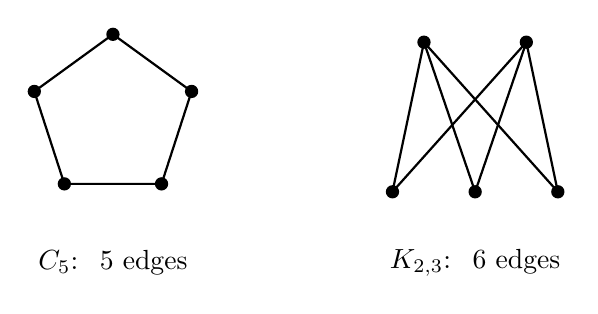
\begin{tikzpicture}[thick]
            \foreach \i in {0,...,4} \coordinate (c\i) at (90+72*\i:1.05);
            \draw (c0) -- (c1) -- (c2) -- (c3) -- (c4) -- (c0);
            \foreach \i in {0,...,4} \fill (c\i) circle (2.4pt);
            \node at (0,-1.85) {$C_5$: \ $5$ edges};
            \begin{scope}[xshift=4.6cm]
                \coordinate (u1) at (-0.65,0.95); \coordinate (u2) at (0.65,0.95);
                \coordinate (w1) at (-1.05,-0.95); \coordinate (w2) at (0,-0.95); \coordinate (w3) at (1.05,-0.95);
                \foreach \u in {u1,u2} \foreach \w in {w1,w2,w3} \draw (\u) -- (\w);
                \foreach \p in {u1,u2,w1,w2,w3} \fill (\p) circle (2.4pt);
                \node at (0,-1.85) {$K_{2,3}$: \ $6$ edges};
            \end{scope}
        \end{tikzpicture}
    \end{center}
\end{eg}

So the greedy algorithm computes a \emph{maximal} \(H\)-free graph rather than a maximum one, and it is natural to ask how few edges a maximal \(H\)-free graph can have.

\begin{definition}[Saturated graph]\label{def:saturated}
    Given a fixed graph \(H\), a graph \(G\) is \vocab{\(H\)-saturated} if
    \begin{enumerate}[(1)]
        \item \(G\) is \(H\)-free, and
        \item adding any missing edge to \(G\) creates a copy of \(H\),
    \end{enumerate}
    i.e.\ \(G\) is maximally \(H\)-free.
\end{definition}

\begin{observation}
    \(G\) is \(H\)-saturated \(\iff\) \(G\) is the output of the \(H\)-free greedy algorithm for some ordering of the edges of \(K_n\).
\end{observation}

\begin{proof}
    (\(\Leftarrow\)) The output \(G\) is \(H\)-free by construction. If \(f\) is a missing edge, it was rejected at its turn because adding it to the graph \(G'\) built so far created a copy of \(H\). As \(G' \subseteq G\), that copy is still present in \(G + f\).

    (\(\Rightarrow\)) Order the edges of \(K_n\) so that those of \(G\) come first. Every prefix of \(E(G)\) is a subgraph of the \(H\)-free graph \(G\), so the algorithm accepts all of them. Afterwards the current graph is \(G\), and each remaining edge \(f\) is rejected since \(G + f\) contains a copy of \(H\) by saturation. The output is \(G\).
\end{proof}

\begin{definition}[Saturation number]
    Given a graph \(H\), the \vocab{saturation number} \(\sat(n, H)\) is the minimum number of edges in an \(n\)-vertex \(H\)-saturated graph.
\end{definition}

\begin{remark}[Why the minimum]
    The maximum gives nothing new: it is the Tur\'an number \(\ex(n,H)\) of \autoref{q:turan} again. An \(H\)-saturated graph is \(H\)-free, so has at most \(\ex(n,H)\) edges; conversely an \(H\)-free graph with \(\ex(n,H)\) edges is saturated, as adding any edge leaves too many for an \(H\)-free graph. So \(\sat(n,H) \le e(G) \le \ex(n,H)\), with both ends attained.
\end{remark}

\begin{notation}[Subscripted \(O\)]\label{not:O-subscript}
    A subscript on \(O\) records which parameters the implied constant is allowed to depend on. Thus \(f(n) = O_k(n)\) means: for each fixed \(k\) there is a constant \(C_k\), depending on \(k\) but \emph{not} on \(n\), with \(\abs{f(n)} \le C_k \, n\) for all \(n\). Plain \(O(\cdot)\), as used earlier, allows no such dependence. Dually, \(g(n) = \Omega(n^2)\) means \(g(n) \ge c \, n^2\) for some constant \(c > 0\) and all large \(n\).
\end{notation}

\begin{theorem}[Bollob\'as, 1965]\label{thm:sat}
    For every \(k \ge 2\),
    \[
        \sat(n, K_k) = \binom{n}{2} - \binom{n-k+2}{2} = (k-2)n - \binom{k-1}{2} = O_k(n).
    \]
\end{theorem}

Here \(\sat(n, K_k) = (k-2)n - \binom{k-1}{2} \le (k-2) n\), so \(C_k = k-2\) works: for each fixed \(k\) the saturation number grows only linearly in \(n\), though the slope \(k-2\) grows with \(k\).

\begin{remark}
    Note how far this is from the Tur\'an problem: for \(k \ge 3\) the largest \(K_k\)-free graphs have \(\Omega(n^2)\) edges, whereas the smallest maximal ones have only \(O_k(n)\).
\end{remark}

\begin{remark}[The bound is best possible]\label{rmk:sat-sharp}
    Join a clique \(K_{k-2}\) to an independent set of \(n-k+2\) vertices, i.e.\ put in all edges inside the clique and all edges between the two parts, and none inside the independent set.
    \begin{center}
        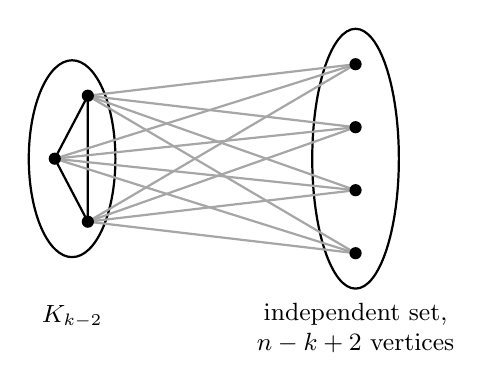
\begin{tikzpicture}[thick, every node/.style={font=\small}]
            \coordinate (a0) at (0.2,0.8); \coordinate (a1) at (-0.22,0); \coordinate (a2) at (0.2,-0.8);
            \draw (a0) -- (a1) -- (a2) -- (a0);
            \draw (0,0) ellipse (0.55 and 1.25);
            \node[align=center] at (0,-2.0) {$K_{k-2}$};
            \foreach \i in {0,1,2,3} \coordinate (b\i) at (3.6,1.2-0.8*\i);
            \draw (3.6,0) ellipse (0.55 and 1.65);
            \node[align=center] at (3.6,-2.15) {independent set,\\$n-k+2$ vertices};
            \foreach \i in {0,1,2} \foreach \j in {0,1,2,3} \draw[gray!70] (a\i) -- (b\j);
            \foreach \i in {0,1,2} \fill (a\i) circle (2.2pt);
            \foreach \i in {0,1,2,3} \fill (b\i) circle (2.2pt);
        \end{tikzpicture}
    \end{center}
    This graph is \(K_k\)-free, since a clique may use at most one vertex of the independent set and so has at most \(k-1\) vertices; and adding any missing edge, which joins two vertices of the independent set, completes a \(K_k\). Its number of edges is
    \[
        \binom{k-2}{2} + (k-2)(n-k+2) = \binom{n}{2} - \binom{n-k+2}{2},
    \]
    so \(\sat(n, K_k)\) is at most the claimed value.
\end{remark}

It remains to prove the matching lower bound, and this is where set pairs enter: the missing edges of a saturated graph, together with the cliques they complete, form a set-pair system.

\begin{proof}[Proof of the lower bound in \autoref{thm:sat}]
    Let \(G\) be a smallest \(K_k\)-saturated graph on \(n\) vertices, and let \(e_1, e_2, \ldots, e_m\) be its missing edges, so that
    \[
        m = \binom{n}{2} - e(G).
    \]
    We construct a set-pair system. Put \(A_i = e_i\), a set of two vertices. By saturation, adding \(e_i\) to \(G\) creates a \(k\)-clique, say on the vertex set \(S_i\) with \(\abs{S_i} = k\); this clique must use the new edge, since \(G\) itself is \(K_k\)-free, so \(e_i \subseteq S_i\). Put \(B_i = V(G) \setminus S_i\), a set of \(n - k\) vertices.
    \begin{center}
        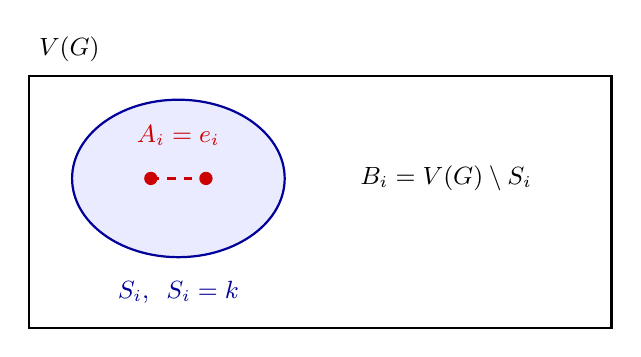
\begin{tikzpicture}[thick, every node/.style={font=\small}]
            \draw (0,0) rectangle (7.4,3.2);
            \node[anchor=south west] at (0,3.25) {$V(G)$};
            \fill[blue!8] (1.9,1.9) ellipse (1.35 and 1.0);
            \draw[blue!60!black] (1.9,1.9) ellipse (1.35 and 1.0);
            \node[blue!60!black] at (1.9,0.45) {$S_i$, \ $\abs{S_i} = k$};
            \fill[red!80!black] (1.55,1.9) circle (2.4pt);
            \fill[red!80!black] (2.25,1.9) circle (2.4pt);
            \draw[red!80!black, dashed] (1.55,1.9) -- (2.25,1.9);
            \node[red!80!black] at (1.9,2.45) {$A_i = e_i$};
            \node at (5.3,1.9) {$B_i = V(G) \setminus S_i$};
        \end{tikzpicture}
    \end{center}
    We check the two conditions of \autoref{def:set-pair}.
    \begin{itemize}
        \item \(A_i \cap B_i = e_i \cap (V(G) \setminus S_i) = \emptyset\), since \(e_i \subseteq S_i\).
        \item Let \(i \ne j\) and suppose \(A_i \cap B_j = \emptyset\), i.e.\ \(e_i \subseteq S_j\). Adding \(e_j\) to \(G\) makes \(S_j\) a clique, so every pair inside \(S_j\) lies in \(E(G) \cup \{e_j\}\). But \(e_i\) is a pair inside \(S_j\) that is neither an edge of \(G\) nor equal to \(e_j\), so it is still missing and \(S_j\) is not a clique in \(G + e_j\). Contradiction; hence \(A_i \cap B_j \ne \emptyset\).
    \end{itemize}
    Thus \(\{(A_i, B_i) : 1 \le i \le m\}\) is a set-pair system with \(\abs{A_i} = 2\) and \(\abs{B_i} = n - k\) for all \(i\), and \autoref{thm:bollobas} gives
    \[
        m \le \binom{2 + (n - k)}{2} = \binom{n-k+2}{2}
        \implies e(G) = \binom{n}{2} - m \ge \binom{n}{2} - \binom{n-k+2}{2}. \qedhere
    \]
\end{proof}

\begin{remark}\hfill
    \begin{enumerate}[(1)]
        \item The same argument works for complete hypergraphs, with \(A_i\) the missing edge and \(B_i\) the complement of the clique it completes.
        \item \vocab{Weak saturation} asks instead that the missing edges can be added one by one \emph{in some order}, each addition creating a new copy of \(H\). Running the argument above only gives the weaker conditions
        \[
            A_i \cap B_i = \emptyset, \qquad A_i \cap B_j \ne \emptyset \ \text{ for } i < j,
        \]
        i.e.\ condition (2) of \autoref{def:set-pair} is required for one of the two orders only. It is still true that \(m \le \binom{k+\ell}{k}\) for such a \emph{skew} set-pair system, but the random-ordering proof breaks down, because the events \(E_i\) are no longer pairwise disjoint, and the only known proofs are algebraic.
        \begin{center}
            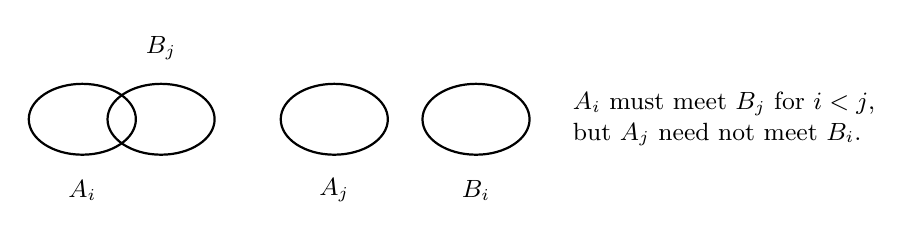
\begin{tikzpicture}[thick, every node/.style={font=\small}]
                \draw (0,0) ellipse (0.68 and 0.45);
                \node at (0,-0.9) {$A_i$};
                \draw (1.0,0) ellipse (0.68 and 0.45);
                \node at (1.0,0.9) {$B_j$};
                \draw (3.2,0) ellipse (0.68 and 0.45);
                \node at (3.2,-0.9) {$A_j$};
                \draw (5.0,0) ellipse (0.68 and 0.45);
                \node at (5.0,-0.9) {$B_i$};
                \node[anchor=west, align=left] at (6.1,0)
                    {\(A_i\) must meet \(B_j\) for \(i < j\),\\but \(A_j\) need not meet \(B_i\).};
            \end{tikzpicture}
        \end{center}
    \end{enumerate}
\end{remark}
